\documentclass[12pt]{article}
\usepackage[T2A]{fontenc}
\usepackage[utf8]{inputenc}
\usepackage{multirow}
\usepackage{caption}
\usepackage{subcaption}
\usepackage{amsmath}
\usepackage{changepage}
\usepackage{graphicx}
\usepackage{float}
\usepackage[english,russian]{babel}
\usepackage{amsmath, amsfonts, amssymb, amsthm, mathtools}
\usepackage{xcolor}
\usepackage{array}
\usepackage{hyperref}
\usepackage{icomma}
\usepackage{mathtext} 
\usepackage[top = 1.5cm, left = 1.5 cm, right = 1.5 cm, bottom = 3 cm]{geometry}
\graphicspath{ {./images/} }
 
\title{Магнитометр}
\author{Шахматов Андрей, Б02-304}
\date{\today}
  
\begin{document}
\begin{titlepage}
    \begin{center}
        {\large МОСКОВСКИЙ ФИЗИКО-ТЕХНИЧЕСКИЙ ИНСТИТУТ (НАЦИОНАЛЬНЫЙ ИССЛЕДОВАТЕЛЬСКИЙ УНИВЕРСИТЕТ)}
    \end{center}
    \begin{center}
        {\large Физтех-школа физики и исследований им. Ландау}
    \end{center}

    \vspace{3cm}
    {\huge
        \begin{center}
            \textbf{Магнитометр}
        \end{center}
    }
    \vspace{2cm}
    \begin{flushright}
        {\LARGE Автор:\\ Шахматов Андрей Юрьевич \\
            \vspace{0.2cm}
            Б02-304}
    \end{flushright}
    \vspace{7 cm}
    \begin{center}
        Долгопрудный 2024
    \end{center}
    \thispagestyle{empty}
\end{titlepage}

% \maketitle

\begin{abstract}
    По влиянию намагниченного стержня на магнитометр определена горизонтальная компонента магнитного поля Земли. При помощи измерения 
    силы тока в разных системах исчисления определена электродинамическая постоянная.
\end{abstract}

% \tableofcontents

\section{Введение}
Цель работы заключается в определении горизонтальной составляющей магнитого поля Земли $B_0$, а так же в 
расчёте электродинамической постоянной $c$.

\section{Методика}
В работе используется магнитометр (Рис. \ref{pic:scheme}). В отсутствии других магнитных полей 
стрелка магнитометра располагается по направлению горизонтальной 
составляющей земного магнитного поля $B_0$. 
 
\begin{figure}[H]
    \centering
    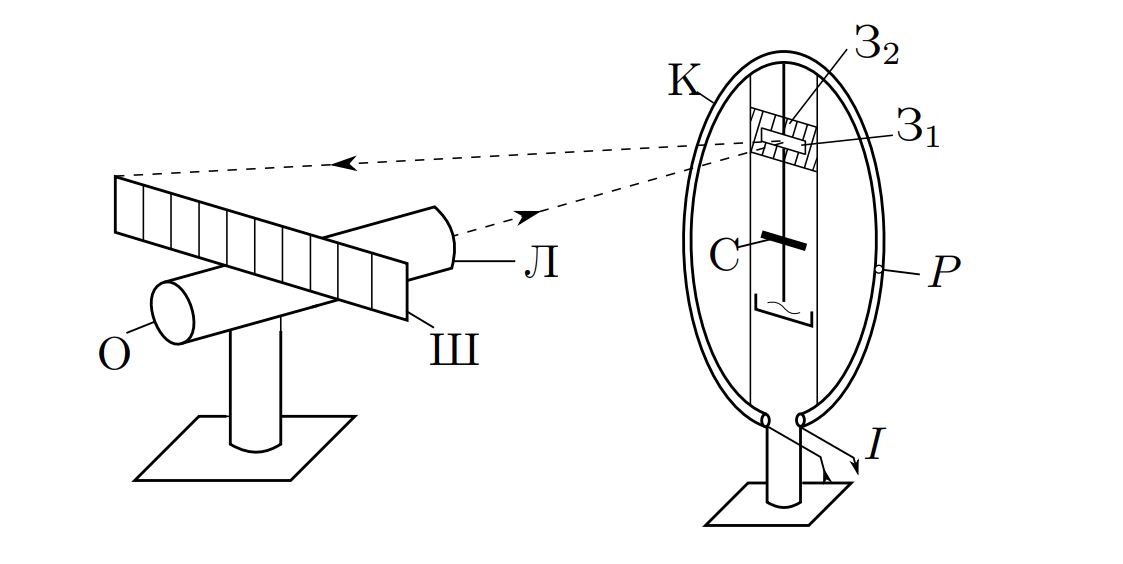
\includegraphics[width=0.6\textwidth]{scheme1.png}
    \caption{Схема магнитометра. Буквами обозначены 
    К --- последовательно соединённые круговые витки, 
    P --- отверстие для установки намагниченного стержня, 
    З --- зеркало, отражающее свет из осветителя О на измерительную 
    шкалу Ш согласно стрелки С, поворачивающейся по направлению магнитного поля
    }
    \label{pic:scheme}
\end{figure}

Если в центре магнитрометра создаётся дополнительное магнитное поле $B$, его стрелка отклонится на 
угол $\varphi$ (Рис. \ref{pic:scheme2}):
\[
    \varphi \approx \tg{\varphi} = \frac{x}{2L}.
\] 
Тогда можно вычислить магнитное поле, вызвавшее отклонение, как 
\[
    B = B_0 \tg \varphi.
\]
\begin{figure}[H]
    \centering
    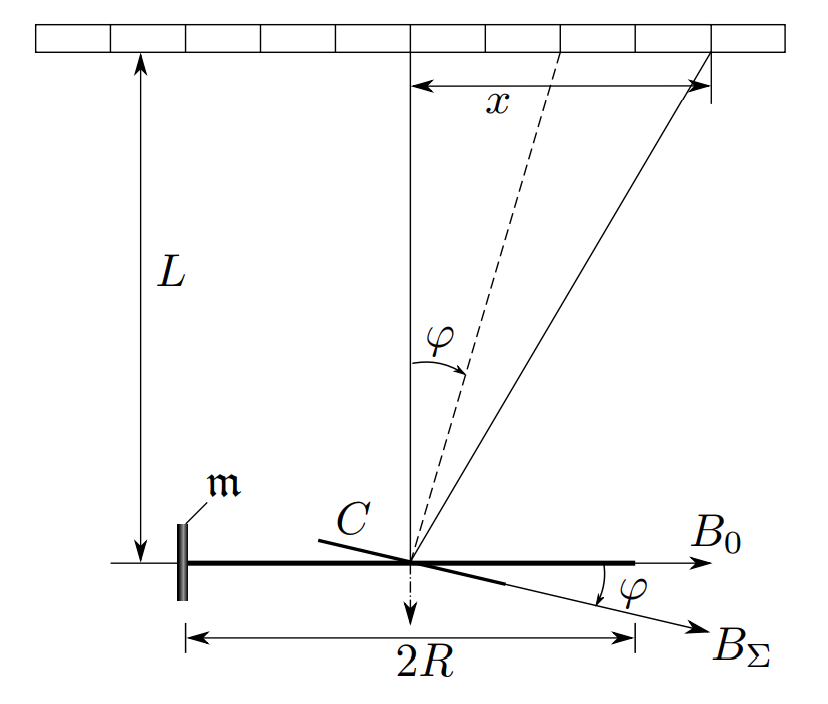
\includegraphics[width=0.4\textwidth]{scheme2.png}
    \caption{Схема измерения угла отклонения магнитной стрелки}
    \label{pic:scheme2}
\end{figure}

\subsection{Определение горизонтальной составляющей магнитного поля Земли}
При помощи намагниченного стержня можно создать дополнительное поле, которое в проекции на ось, перпендикулярную стрежню, описывается выражением
\[
    B_1 = \frac{\mu_0}{4 \pi } \frac{m}{R^3},
\]
где $m$ --- магнитный момент стержня, $R$ --- радиус кольца. 
Дополнительно, при помощи измерения крутильных колебаний стержня в магнитном поле найдём магнитный момент стрежня. 
Крутильные колебания диполя можно описать уравнением
\[
    J \ddot \alpha + m B_0 \alpha  = 0,
\]
где $J = \frac{ml^2}{12} \left[ 1 + 3 \left( \frac{r}{l} \right)^2  \right] $ --- момент инерции стрежня. Из решения уравенения следует, что 
период колебаний вычисляется как 
\[
    T = 2 \pi \sqrt{\frac{J}{mB_0}},
\]  
В таком случае можно получить выражение для горизонтальной составляющей магнитного поля Земли 
\[
    B_0 = \frac{2 \pi }{TR} \sqrt{\frac{\mu_0 J L}{2 \pi R x_1}}.
\]

\subsection{Определение электродинамической постоянной}
Если пропустить ток по виткам магнитрометра, в центре создастся магнитное поле $B_2$:
\[
    B_2 = \frac{\mu_0 I}{2 R} N, 
\] 
где $N$ --- число витков в кольце, $I$ --- сила тока в единицах СИ.  
В таком случае можно выразить ток $I$ через угол отклонения магнитометра как 
\[
    I = \frac{2 B_0 R}{\mu_0 N} \frac{x_2}{2L}.
\] 
Также можно измерить ток абсолютным способом, как заряд, прошедший с конденсатора через кольцо в единицу времени: 
\[
    I = CU\nu,
\]
где $C$ --- ёмкость конденсатора в единицах СГС, $U$ --- напряжение источника в единицах СГС, $\nu$ --- частота источника.  
Таким образом можно вычислить электродинамическую постоянную в единицах СИ как 
\[
    c = \frac{1}{10} \frac{I_{[\textrm{СГС}]}}{I_{[\textrm{СИ}]}}.
\]

\section{Результаты и их обсуждение}

Измерено отклонение магнитометра $x_1 = 4,0 \pm 0,5$ см от воздействия намагниченного стержня. 
После определён период малых крутильных колебаний стержня, путём измерения $10$ колебаний и последующего усреднения, 
период составил $T = 10,9 \pm 0,2$ с. 

При использованием штангенциркуля определены размеры намагниченного стержня 
$d = 4,9 \pm 0,1$ мм --- диаметр стержня, $l = 39,9 \pm 0,1$ мм --- длина стержня. Вычислен момент инерции стержня
\[
    J = (5.70 \pm 0.04) \cdot 10^{-7} \textrm{ кг} \cdot \textrm{м}^2.
\]  

Согласно параметрам установки (Прил. \ref{app_1}) и измеренным выше значениям, вычислена горизонтальная компонента 
магнитного поля Земли: 
\[
    B_0 = (1.14 \pm 0.09) \cdot 10^{-5} \textrm{ Тл}. 
\]

После подачи тока на кольцо магнитометра, измерено отклонение стрелки $x_2 = 13,5 \pm 0,5$ см.  
Тогда ток, измеренный в единицах СИ
\[
    I_{[\textrm{СИ}]} = (5.1 \pm 0.4) \cdot 10^{-3} \textrm{ А}.
\]
Тогда как ток, измеренный в СГС 
\[
    I_{[\textrm{СГС}]} = (1.48 \pm 0.12) \cdot 10^7 \textrm{ ед. СГС}.
\]
Электродинамическая постоянная получается из отношение этих токов
\[
    c = (2.91 \pm 0.32) \cdot 10^8 \, \frac{\textrm{м}}{\textrm{с}^2}.
\]

\section{Выводы}
Определена горизонтальная составляющая магнитного поля Земли $B_0 = (1.14 \pm 0.09) \cdot 10^{-5} \textrm{ Тл}$, 
что совпадает по порядку с табличным значением магнитного поля Земли $B \approx 30$ мкТл. 
Определено значение электродинамической постоянной $c = (2.91 \pm 0.32) \cdot 10^8 \, \frac{\textrm{м}}{\textrm{с}^2}$, 
что совпадает с табличным значением $c \approx 3 \cdot 10^8 \, \frac{\textrm{м}}{\textrm{с}^2}$ в пределах погрешности.


\section{Использованная литература}
\begin{thebibliography}{9}
    \bibitem{LabBook}
    Лабораторный практикум по общей физике, Том 2, под редакцией А. Д. Гладуна
\end{thebibliography}

\section{Приложения}
\subsection{Параметры установки и погрешности приборов} \label{app_1}
$L = 110 \pm 1$ см --- расстояние от осветителя до зеркала,
$D = 40 \pm 1$ см --- диаметр кольца магнитометра,
$C = (9,00 \pm 0,18) \cdot 10^5$ см --- ёмкость конденсатора в СГС,
$U = 98,6 \pm 0,3$ В --- напряжение источника,
$m = 4,25$ г --- масса стержня,
$n = 50$ Гц --- частота источника. 


\end{document}